%---------------------------------------
\addcontentsline{toc}{chapter}{1 Corinthians}

% Safely inserts your illustration full-bleed on its own page.
% This completely bypasses the page builder, headers, and geometry bugs!
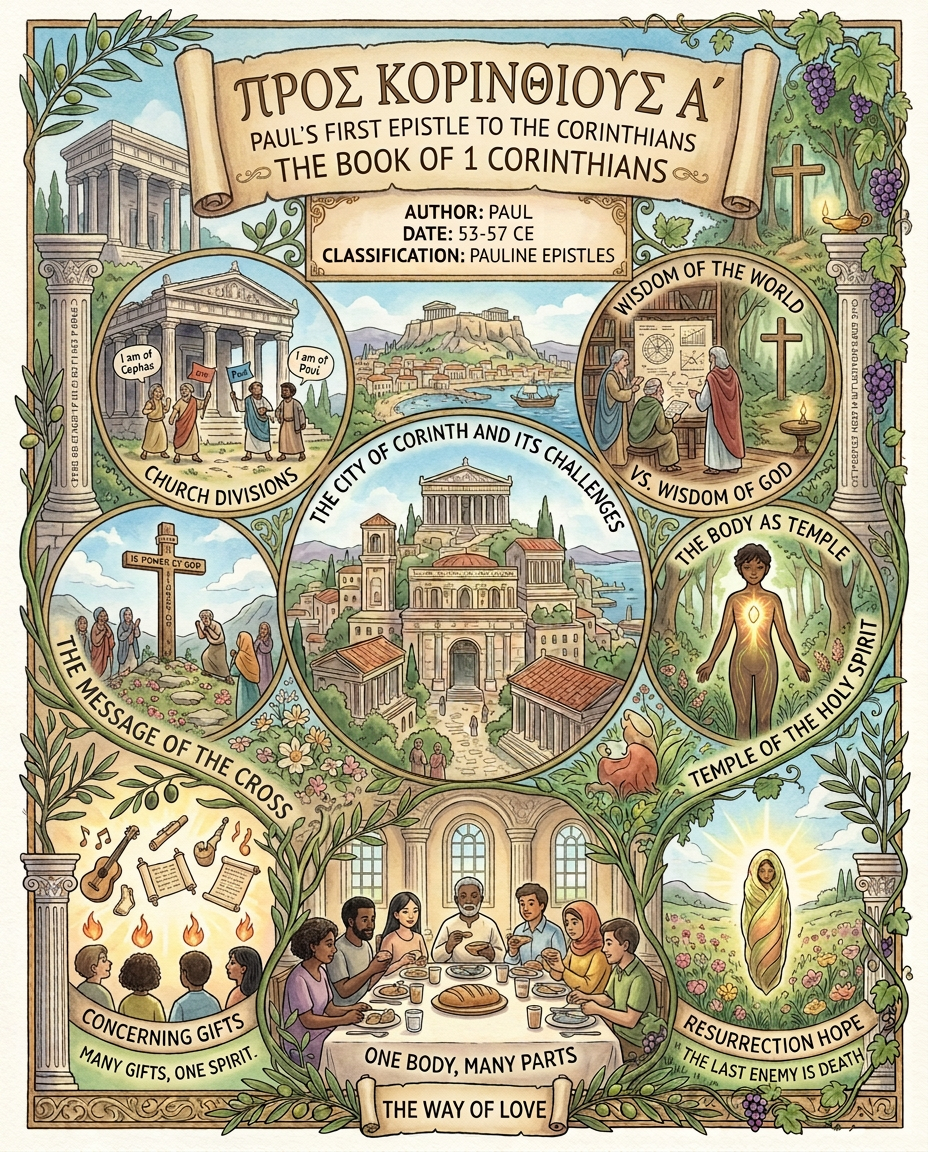
\includepdf[pages=1, fitpaper=false, width=\paperwidth, height=\paperheight, , keepaspectratio=false]{images/divider2/1corinthians2.png}
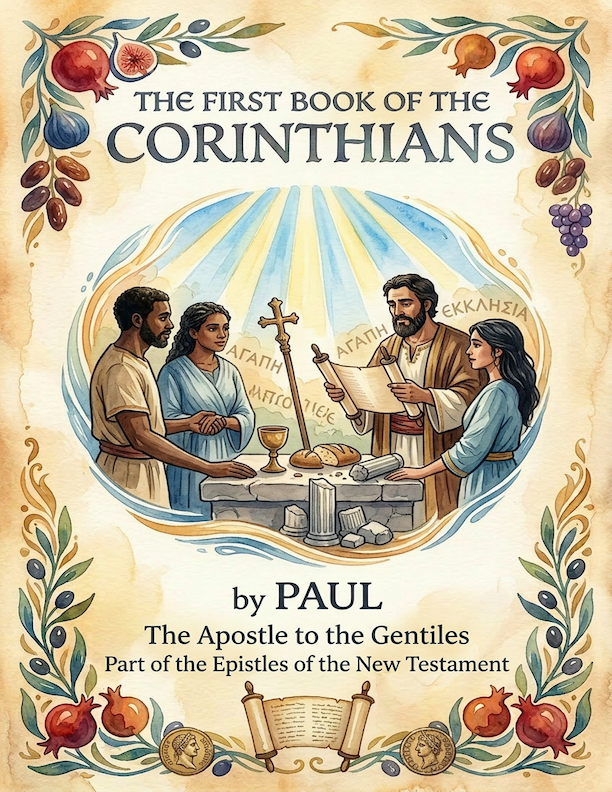
\includepdf[pages=1, fitpaper=false, width=\paperwidth, height=\paperheight, , keepaspectratio=false]{images/divider1/1corinthians.png}

\includepdf[pages=1, fitpaper=false, width=\paperwidth, height=\paperheight, , keepaspectratio=false]{images/8.5x11-Dot-Grid.png}

\includepdf[pages=1, fitpaper=false, width=\paperwidth, height=\paperheight, , keepaspectratio=false]{images/8.5x11-Dot-Grid.png}

\mybook{1 Corinthians}
\vspace{-1.36in}


\mychapter{} \myverse*{}Paul, called to be an emissary of Yeshua the Messiah\footnote{1:1 “Messiah” means “Anointed One”.} through the will of God, and our brother Sosthenes,
\myverse{}to the assembly of God which is at Corinth—those who are sanctified in Messiah
Yeshua, called holy ones, with all who call on the name of our Lord Yeshua the Messiah in every place,
both theirs and ours:
\myverse{}Grace to you and peace from God our Father and the Lord Yeshua the Messiah.

\myverse{}I always thank my God concerning you for the grace of God which
was given you in Messiah Yeshua,
\myverse{}that in everything you were enriched in him, in all speech and all knowledge—
\myverse{}even as the testimony of Messiah was confirmed in you—
\myverse{}so that you come behind in no gift, waiting for the revelation of our Lord Yeshua the Messiah,
\myverse{}who will also confirm you until the end, blameless in the day of our Lord Yeshua the Messiah.
\myverse{}God is faithful, through whom you were called into the fellowship of his Son,
Yeshua the Messiah our Lord.

\myverse{}Now I beg you, brothers,\footnote{1:10 The word for “brothers” here and where context allows may also be correctly translated “brothers
	and sisters” or “siblings.”} through the name of our Lord, Yeshua the Messiah, that you all speak
the same thing, and that there be no divisions among you, but that you be perfected together in the same
mind and in the same judgment.
\myverse{}For it has been reported to me concerning you, my brothers, by those who are
from Chloe’s household, that there are contentions among you.
\myverse{}Now I mean this, that each one of you says, “I follow Paul,” “I follow Apollos,”
“I follow Kefa,” and, “I follow Messiah.”
\myverse{}Is Messiah divided? Was Paul crucified for you? Or were you immersed into
the name of Paul?
\myverse{}I thank God that I immersed none of you except Crispus and Gaius,
\myverse{}so that no one should say that I had immersed you into my own name.
\myverse{}(I also immersed the household of Stephanas; besides them, I don’t know whether
I immersed any other.)
\myverse{}For Messiah sent me not to immerse, but to proclaim the Good News—not in wisdom
of words, so that the cross of Messiah wouldn’t be made void.
\myverse{}For the word of the cross is foolishness to those who are dying, but to us
who are being saved it is the power of God.
\myverse{}For it is written,

“I will destroy the wisdom of the wise.

I will bring the discernment of the discerning to nothing.”\footnote{1:19 Isaiah 29:14}

\myverse{}Where is the wise? Where is the scribe? Where is the debater
of this age? Hasn’t God made foolish the wisdom of this world?
\myverse{}For seeing that in the wisdom of God, the world through its wisdom didn’t
know God, it was God’s good pleasure through the foolishness of the proclaiming to save those who believe.
\myverse{}For Jews ask for signs, Greeks seek after wisdom,
\myverse{}but we proclaim Messiah crucified, a stumbling block to Jews and foolishness
to Greeks,
\myverse{}but to those who are called, both Jews and Greeks, Messiah is the power of
God and the wisdom of God;
\myverse{}because the foolishness of God is wiser than men, and the weakness of God
is stronger than men.

\myverse{}For you see your calling, brothers, that not many are wise according
to the flesh, not many mighty, and not many noble;
\myverse{}but God chose the foolish things of the world that he might put to shame those
who are wise. God chose the weak things of the world that he might put to shame the things that are strong.
\myverse{}God chose the lowly things of the world, and the things that are despised,
and the things that don’t exist, that he might bring to nothing the things that exist,
\myverse{}that no flesh should boast before God.
\myverse{}Because of him, you are in Messiah Yeshua, who was made to us wisdom from
God, and righteousness and sanctification, and redemption,
\myverse{}that, as it is written, “He who boasts, let him boast in the Lord.”\footnote{1:31 Jeremiah 9:24}


% 1 CORINTHIANS 2
\mychapter{} \myverse*{}When I came to you, brothers, I didn’t come with excellence of
speech or of wisdom, proclaiming to you the testimony of God.
\myverse{}For I determined not to know anything among you except Yeshua the Messiah and
him crucified.
\myverse{}I was with you in weakness, in fear, and in much trembling.
\myverse{}My speech and my proclaiming were not in persuasive words of human wisdom, but
in demonstration of the Spirit and of power,
\myverse{}that your faith wouldn’t stand in the wisdom of men, but in the power of God.

\myverse{}We speak wisdom, however, among those who are full grown, yet a
wisdom not of this world nor of the rulers of this world who are coming to nothing.
\myverse{}But we speak God’s wisdom in a mystery, the wisdom that has been hidden, which
God foreordained before the worlds for our glory,
\myverse{}which none of the rulers of this world has known. For had they known it, they
wouldn’t have crucified the Lord of glory.
\myverse{}But as it is written,

“Things which an eye didn’t see, and an ear didn’t hear,

which didn’t enter into the heart of man,

these God has prepared for those who love him.”\footnote{2:9 Isaiah 64:4}

\myverse{}But to us, God revealed them through the Spirit. For the Spirit
searches all things, yes, the deep things of God.
\myverse{}For who among men knows the things of a man except the spirit of the man which
is in him? Even so, no one knows the things of God except God’s Spirit.
\myverse{}But we received not the spirit of the world, but the Spirit which is from
God, that we might know the things that were freely given to us by God.
\myverse{}We also speak these things, not in words which man’s wisdom teaches but which
the Holy Spirit teaches, comparing spiritual things with spiritual things.
\myverse{}Now the natural man doesn’t receive the things of God’s Spirit, for they are
foolishness to him; and he can’t know them, because they are spiritually discerned.
\myverse{}But he who is spiritual discerns all things, and he himself is to be judged
by no one.
\myverse{}“For who has known the mind of the Lord that he should instruct him?”\footnote{2:16 Isaiah 40:13} But we have Messiah’s mind.


% 1 CORINTHIANS 3
\mychapter{} \myverse*{}Brothers, I couldn’t speak to you as to spiritual, but as to fleshly,
as to babies in Messiah.
\myverse{}I fed you with milk, not with solid food, for you weren’t yet ready. Indeed,
you aren’t ready even now,
\myverse{}for you are still fleshly. For insofar as there is jealousy, strife, and factions
among you, aren’t you fleshly, and don’t you walk in the ways of men?
\myverse{}For when one says, “I follow Paul,” and another, “I follow Apollos,” aren’t
you fleshly?

\myverse{}Who then is Apollos, and who is Paul, but servants through whom
you believed, and each as the Lord gave to him?
\myverse{}I planted. Apollos watered. But God gave the increase.
\myverse{}So then neither he who plants is anything, nor he who waters, but God who gives
the increase.
\myverse{}Now he who plants and he who waters are the same, but each will receive his
own reward according to his own labor.
\myverse{}For we are God’s fellow workers. You are God’s farming, God’s building.

\myverse{}According to the grace of God which was given to me, as a wise
master builder I laid a foundation, and another builds on it. But let each man be careful how he builds
on it.
\myverse{}For no one can lay any other foundation than that which has been laid, which
is Yeshua the Messiah.
\myverse{}But if anyone builds on the foundation with gold, silver, costly stones, wood,
hay, or straw,
\myverse{}each man’s work will be revealed. For the Day will declare it, because it
is revealed in fire; and the fire itself will test what sort of work each man’s work is.
\myverse{}If any man’s work remains which he built on it, he will receive a reward.
\myverse{}If any man’s work is burned, he will suffer loss, but he himself will be saved,
but as through fire.

\myverse{}Don’t you know that you are God’s temple and that God’s Spirit
lives in you?
\myverse{}If anyone destroys God’s temple, God will destroy him; for God’s temple is
holy, which you are.

\myverse{}Let no one deceive himself. If anyone thinks that he is wise
among you in this world, let him become a fool that he may become wise.
\myverse{}For the wisdom of this world is foolishness with God. For it is written, “He
has taken the wise in their craftiness.”\footnote{3:19 Job 5:13}
\myverse{}And again, “The Lord knows the reasoning of the wise, that it is worthless.”\footnote{3:20 Psalms 94:11}
\myverse{}Therefore let no one boast in men. For all things are yours,
\myverse{}whether Paul, or Apollos, or Kefa, or the world, or life, or death, or things
present, or things to come. All are yours,
\myverse{}and you are Messiah’s, and Messiah is God’s.


% 1 CORINTHIANS 4
\mychapter{} \myverse*{}So let a man think of us as Messiah’s servants and stewards of
God’s mysteries.
\myverse{}Here, moreover, it is required of stewards that they be found faithful.
\myverse{}But with me it is a very small thing that I should be judged by you, or by a
human court. Yes, I don’t even judge my own self.
\myverse{}For I know nothing against myself. Yet I am not justified by this, but he who
judges me is the Lord.
\myverse{}Therefore judge nothing before the time, until the Lord comes, who will both
bring to light the hidden things of darkness and reveal the counsels of the hearts. Then each man will
get his praise from God.

\myverse{}Now these things, brothers, I have in a figure transferred to myself
and Apollos for your sakes, that in us you might learn not to think beyond the things which are written,
that none of you be puffed up against one another.
\myverse{}For who makes you different? And what do you have that you didn’t receive? But
if you did receive it, why do you boast as if you had not received it?

\myverse{}You are already filled. You have already become rich. You have
come to reign without us. Yes, and I wish that you did reign, that we also might reign with you!
\myverse{}For I think that God has displayed us, the emissaries, last of all, like men
sentenced to death. For we are made a spectacle to the world, both to angels and men.
\myverse{}We are fools for Messiah’s sake, but you are wise in Messiah. We are weak,
but you are strong. You have honor, but we have dishonor.
\myverse{}Even to this present hour we hunger, thirst, are naked, are beaten, and have
no certain dwelling place.
\myverse{}We toil, working with our own hands. When people curse us, we bless. Being
persecuted, we endure.
\myverse{}Being defamed, we entreat. We are made as the filth of the world, the dirt
wiped off by all, even until now.

\myverse{}I don’t write these things to shame you, but to admonish you
as my beloved children.
\myverse{}For though you have ten thousand tutors in Messiah, you don’t have many fathers.
For in Messiah Yeshua, I became your father through the Good News.
\myverse{}I beg you therefore, be imitators of me.
\myverse{}Because of this I have sent Timothy to you, who is my beloved and faithful
child in the Lord, who will remind you of my ways which are in Messiah, even as I teach everywhere in
every assembly.
\myverse{}Now some are puffed up, as though I were not coming to you.
\myverse{}But I will come to you shortly, if the Lord is willing. And I will know, not
the word of those who are puffed up, but the power.
\myverse{}For God’s Kingdom is not in word, but in power.
\myverse{}What do you want? Shall I come to you with a rod, or in love and a spirit
of gentleness?


% 1 CORINTHIANS 5
\mychapter{} \myverse*{}It is actually reported that there is sexual immorality among you,
and such sexual immorality as is not even named among the Gentiles, that one has his father’s wife.
\myverse{}You are arrogant, and didn’t mourn instead, that he who had done this deed might
be removed from among you.
\myverse{}For I most certainly, as being absent in body but present in spirit, have already,
as though I were present, judged him who has done this thing.
\myverse{}In the name of our Lord Yeshua the Messiah, when you are gathered together with
my spirit with the power of our Lord Yeshua the Messiah,
\myverse{}you are to deliver such a one to Satan for the destruction of the flesh, that
the spirit may be saved in the day of the Lord Yeshua.

\myverse{}Your boasting is not good. Don’t you know that a little yeast leavens
the whole lump?
\myverse{}Purge out the old yeast, that you may be a new lump, even as you are unleavened.
For indeed Messiah, our Passover, has been sacrificed in our place.
\myverse{}Therefore let’s keep the feast, not with old yeast, neither with the yeast of
malice and wickedness, but with the unleavened bread of sincerity and truth.

\myverse{}I wrote to you in my letter to have no company with sexual sinners;
\myverse{}yet not at all meaning with the sexual sinners of this world, or with the
covetous and extortionists, or with idolaters, for then you would have to leave the world.
\myverse{}But as it is, I wrote to you not to associate with anyone who is called a
brother who is a sexual sinner, or covetous, or an idolater, or a slanderer, or a drunkard, or an extortionist.
Don’t even eat with such a person.
\myverse{}For what do I have to do with also judging those who are outside? Don’t you
judge those who are within?
\myverse{}But those who are outside, God judges. “Put away the wicked man from among
yourselves.”\footnote{5:13 Deuteronomy 17:7;
	19:19;
	21:21;
	22:21;
	24:7}


% 1 CORINTHIANS 6
\mychapter{} \myverse*{}Dare any of you, having a matter against his neighbor, go to law
before the unrighteous, and not before the holy ones?
\myverse{}Don’t you know that the holy ones will judge the world? And if the world is
judged by you, are you unworthy to judge the smallest matters?
\myverse{}Don’t you know that we will judge angels? How much more, things that pertain
to this life?
\myverse{}If then you have to judge things pertaining to this life, do you set them to
judge who are of no account in the assembly?
\myverse{}I say this to move you to shame. Isn’t there even one wise man among you who
would be able to decide between his brothers?
\myverse{}But brother goes to law with brother, and that before unbelievers!
\myverse{}Therefore it is already altogether a defect in you that you have lawsuits one
with another. Why not rather be wronged? Why not rather be defrauded?
\myverse{}No, but you yourselves do wrong and defraud, and that against your brothers.

\myverse{}Or don’t you know that the unrighteous will not inherit God’s Kingdom?
Don’t be deceived. Neither the sexually immoral, nor idolaters, nor adulterers, nor male prostitutes,
nor homosexuals,
\myverse{}nor thieves, nor covetous, nor drunkards, nor slanderers, nor extortionists,
will inherit God’s Kingdom.
\myverse{}Some of you were such, but you were washed. You were sanctified. You were
justified in the name of the Lord Yeshua, and in the Spirit of our God.

\myverse{}“All things are lawful for me,” but not all things are expedient.
“All things are lawful for me,” but I will not be brought under the power of anything.
\myverse{}“Foods for the belly, and the belly for foods,” but God will bring to nothing
both it and them. But the body is not for sexual immorality, but for the Lord, and the Lord for the body.
\myverse{}Now God raised up the Lord, and will also raise us up by his power.
\myverse{}Don’t you know that your bodies are members of Messiah? Shall I then take
the members of Messiah and make them members of a prostitute? May it never be!
\myverse{}Or don’t you know that he who is joined to a prostitute is one body? For,
“The two”, he says, “will become one flesh.”\footnote{6:16 Genesis 2:24}
\myverse{}But he who is joined to the Lord is one spirit.
\myverse{}Flee sexual immorality! “Every sin that a man does is outside the body,” but
he who commits sexual immorality sins against his own body.
\myverse{}Or don’t you know that your body is a temple of the Holy Spirit who is in
you, whom you have from God? You are not your own,
\myverse{}for you were bought with a price. Therefore glorify God in your body and in
your spirit, which are God’s.


% 1 CORINTHIANS 7
\mychapter{} \myverse*{}Now concerning the things about which you wrote to me: it is good
for a man not to touch a woman.
\myverse{}But, because of sexual immoralities, let each man have his own wife, and let
each woman have her own husband.
\myverse{}Let the husband give his wife the affection owed her,\footnote{7:3 NU and TR have “what is owed her” instead of “the affection owed her”.} and likewise
also the wife her husband.
\myverse{}The wife doesn’t have authority over her own body, but the husband does. Likewise
also the husband doesn’t have authority over his own body, but the wife does.
\myverse{}Don’t deprive one another, unless it is by consent for a season, that you may
give yourselves to fasting and prayer, and may be together again, that Satan doesn’t tempt you because
of your lack of self-control.

\myverse{}But this I say by way of concession, not of commandment.
\myverse{}Yet I wish that all men were like me. However, each man has his own gift from
God, one of this kind, and another of that kind.
\myverse{}But I say to the unmarried and to widows, it is good for them if they remain
even as I am.
\myverse{}But if they don’t have self-control, let them marry. For it’s better to marry
than to burn with passion.
\myverse{}But to the married I command—not I, but the Lord—that the wife not leave her
husband
\myverse{}(but if she departs, let her remain unmarried, or else be reconciled to her
husband), and that the husband not leave his wife.

\myverse{}But to the rest I—not the Lord—say, if any brother has an unbelieving
wife, and she is content to live with him, let him not leave her.
\myverse{}The woman who has an unbelieving husband, and he is content to live with her,
let her not leave her husband.
\myverse{}For the unbelieving husband is sanctified in the wife, and the unbelieving
wife is sanctified in the husband. Otherwise your children would be unclean, but now they are holy.
\myverse{}Yet if the unbeliever departs, let there be separation. The brother or the
sister is not under bondage in such cases, but God has called us in peace.
\myverse{}For how do you know, wife, whether you will save your husband? Or how do you
know, husband, whether you will save your wife?

\myverse{}Only, as the Lord has distributed to each man, as God has called
each, so let him walk. So I command in all the assemblies.

\myverse{}Was anyone called having been circumcised? Let him not become
uncircumcised. Has anyone been called in uncircumcision? Let him not be circumcised.
\myverse{}Circumcision is nothing, and uncircumcision is nothing, but what matters is
keeping God’s commandments.
\myverse{}Let each man stay in that calling in which he was called.
\myverse{}Were you called being a bondservant? Don’t let that bother you, but if you
get an opportunity to become free, use it.
\myverse{}For he who was called in the Lord being a bondservant is the Lord’s free man.
Likewise he who was called being free is Messiah’s bondservant.
\myverse{}You were bought with a price. Don’t become bondservants of men.
\myverse{}Brothers, let each man, in whatever condition he was called, stay in that
condition with God.

\myverse{}Now concerning virgins, I have no commandment from the Lord,
but I give my judgment as one who has obtained mercy from the Lord to be trustworthy.
\myverse{}Therefore I think that because of the distress that is on us, it’s good for
a man to remain as he is.
\myverse{}Are you bound to a wife? Don’t seek to be freed. Are you free from a wife?
Don’t seek a wife.
\myverse{}But if you marry, you have not sinned. If a virgin marries, she has not sinned.
Yet such will have oppression in the flesh, and I want to spare you.
\myverse{}But I say this, brothers: the time is short. From now on, both those who have
wives may be as though they had none;
\myverse{}and those who weep, as though they didn’t weep; and those who rejoice, as
though they didn’t rejoice; and those who buy, as though they didn’t possess;
\myverse{}and those who use the world, as not using it to the fullest. For the mode
of this world passes away.

\myverse{}But I desire to have you to be free from cares. He who is unmarried
is concerned for the things of the Lord, how he may please the Lord;
\myverse{}but he who is married is concerned about the things of the world, how he may
please his wife.
\myverse{}There is also a difference between a wife and a virgin. The unmarried woman
cares about the things of the Lord, that she may be holy both in body and in spirit. But she who is married
cares about the things of the world—how she may please her husband.
\myverse{}This I say for your own benefit, not that I may ensnare you, but for that
which is appropriate, and that you may attend to the Lord without distraction.

\myverse{}But if any man thinks that he is behaving inappropriately toward
his virgin, if she is past the flower of her age, and if need so requires, let him do what he desires.
He doesn’t sin. Let them marry.
\myverse{}But he who stands steadfast in his heart, having no urgency, but has power
over his own will, and has determined in his own heart to keep his own virgin, does well.
\myverse{}So then both he who gives his own virgin in marriage does well, and he who
doesn’t give her in marriage does better.

\myverse{}A wife is bound by law for as long as her husband lives; but
if the husband is dead, she is free to be married to whomever she desires, only in the Lord.
\myverse{}But she is happier if she stays as she is, in my judgment, and I think that
I also have God’s Spirit.


%1 CORINTHIANS 8
\mychapter{} \myverse*{}Now concerning things sacrificed to idols: We know that we all
have knowledge. Knowledge puffs up, but love builds up.
\myverse{}But if anyone thinks that he knows anything, he doesn’t yet know as he ought
to know.
\myverse{}But anyone who loves God is known by him.

\myverse{}Therefore concerning the eating of things sacrificed to idols,
we know that no idol is anything in the world, and that there is no other God but one.
\myverse{}For though there are things that are called “gods”, whether in the heavens or
on earth—as there are many “gods” and many “lords”—
\myverse{}yet to us there is one God, the Father, of whom are all things, and we for him;
and one Lord, Yeshua the Messiah, through whom are all things, and we live through him.

\myverse{}However, that knowledge isn’t in all men. But some, with consciousness
of an idol until now, eat as of a thing sacrificed to an idol, and their conscience, being weak, is defiled.
\myverse{}But food will not commend us to God. For neither, if we don’t eat are we the
worse, nor if we eat are we the better.
\myverse{}But be careful that by no means does this liberty of yours become a stumbling
block to the weak.
\myverse{}For if a man sees you who have knowledge sitting in an idol’s temple, won’t
his conscience, if he is weak, be emboldened to eat things sacrificed to idols?
\myverse{}And through your knowledge, he who is weak perishes, the brother for whose
sake Messiah died.
\myverse{}Thus, sinning against the brothers, and wounding their conscience when it
is weak, you sin against Messiah.
\myverse{}Therefore, if food causes my brother to stumble, I will eat no meat forever
more, that I don’t cause my brother to stumble.


%1 CORINTHIANS 9
\mychapter{} \myverse*{}Am I not free? Am I not an emissary? Haven’t I seen Yeshua the Messiah,
our Lord? Aren’t you my work in the Lord?
\myverse{}If to others I am not an emissary, yet at least I am to you; for you are the
seal of my office of emissary in the Lord.

\myverse{}My defense to those who examine me is this:
\myverse{}Have we no right to eat and to drink?
\myverse{}Have we no right to take along a wife who is a believer, even as the rest of
the emissaries, and the brothers of the Lord, and Kefa?
\myverse{}Or have only Barnabas and I no right to not work?
\myverse{}What soldier ever serves at his own expense? Who plants a vineyard, and doesn’t
eat of its fruit? Or who feeds a flock, and doesn’t drink from the flock’s milk?

\myverse{}Do I speak these things according to the ways of men? Or doesn’t
the Torah also say the same thing?
\myverse{}For it is written in the Torah of Moses, “You shall not muzzle an ox while it
treads out the grain.”\footnote{9:9 Deuteronomy 25:4} Is it for the oxen that God cares,
\myverse{}or does he say it assuredly for our sake? Yes, it was written for our sake,
because he who plows ought to plow in hope, and he who threshes in hope should partake of his hope.
\myverse{}If we sowed to you spiritual things, is it a great thing if we reap your fleshly
things?
\myverse{}If others partake of this right over you, don’t we yet more?

Nevertheless we didn’t use this right, but we bear all things, that we may cause no hindrance
to the Good News of Messiah.
\myverse{}Don’t you know that those who serve around sacred things eat from the things
of the temple, and those who wait on the altar have their portion with the altar?
\myverse{}Even so the Lord ordained that those who proclaim the Good News should live
from the Good News.

\myverse{}But I have used none of these things, and I don’t write these
things that it may be done so in my case; for I would rather die, than that anyone should make my boasting
void.
\myverse{}For if I proclaim the Good News, I have nothing to boast about, for necessity
is laid on me; but woe is to me if I don’t proclaim the Good News.
\myverse{}For if I do this of my own will, I have a reward. But if not of my own will,
I have a stewardship entrusted to me.
\myverse{}What then is my reward? That when I proclaim the Good News, I may present
the Good News of Messiah without charge, so as not to abuse my authority in the Good News.

\myverse{}For though I was free from all, I brought myself under bondage
to all, that I might gain the more.
\myverse{}To the Jews I became as a Jew, that I might gain Jews; to those who are under
the law, as under the law,\footnote{9:20 NU adds: though I myself am not under the law} that I might gain those who are under
the law;
\myverse{}to those who are without law, as without law (not being without law toward
God, but under law toward Messiah), that I might win those who are without law.
\myverse{}To the weak I became as weak, that I might gain the weak. I have become all
things to all men, that I may by all means save some.
\myverse{}Now I do this for the sake of the Good News, that I may be a joint partaker
of it.
\myverse{}Don’t you know that those who run in a race all run, but one receives the
prize? Run like that, so that you may win.
\myverse{}Every man who strives in the games exercises self-control in all things. Now
they do it to receive a corruptible crown, but we an incorruptible.
\myverse{}I therefore run like that, not aimlessly. I fight like that, not beating the
air,
\myverse{}but I beat my body and bring it into submission, lest by any means, after
I have preached to others, I myself should be disqualified.


% 1 CORINTHIANS 10
\mychapter{} \myverse*{}Now I would not have you ignorant, brothers, that our fathers
were all under the cloud, and all passed through the sea;
\myverse{}and were all immersed into Moses in the cloud and in the sea;
\myverse{}and all ate the same spiritual food;
\myverse{}and all drank the same spiritual drink. For they drank of a spiritual rock
that followed them, and the rock was Messiah.
\myverse{}However with most of them, God was not well pleased, for they were overthrown
in the wilderness.

\myverse{}Now these things were our examples, to the intent we should not
lust after evil things as they also lusted.
\myverse{}Don’t be idolaters, as some of them were. As it is written, “The people sat
down to eat and drink, and rose up to play.”\footnote{10:7 Exodus 32:6}
\myverse{}Let’s not commit sexual immorality, as some of them committed, and in one day
twenty-three thousand fell.
\myverse{}Let’s not test Messiah,\footnote{10:9 NU reads “the Lord” instead of “Messiah”.} as some of them tested, and perished by the
serpents.
\myverse{}Don’t grumble, as some of them also grumbled, and perished by the destroyer.
\myverse{}Now all these things happened to them by way of example, and they were written
for our admonition, on whom the ends of the ages have come.
\myverse{}Therefore let him who thinks he stands be careful that he doesn’t fall.

\myverse{}No temptation has taken you except what is common to man. God
is faithful, who will not allow you to be tempted above what you are able, but will with the temptation
also make the way of escape, that you may be able to endure it.

\myverse{}Therefore, my beloved, flee from idolatry.
\myverse{}I speak as to wise men. Judge what I say.
\myverse{}The cup of blessing which we bless, isn’t it a sharing of the blood of Messiah?
The bread which we break, isn’t it a sharing of the body of Messiah?
\myverse{}Because there is one loaf of bread, we, who are many, are one body; for we
all partake of the one loaf of bread.
\myverse{}Consider Israel according to the flesh. Don’t those who eat the sacrifices
participate in the altar?

\myverse{}What am I saying then? That a thing sacrificed to idols is anything,
or that an idol is anything?
\myverse{}But I say that the things which the Gentiles sacrifice, they sacrifice to
demons and not to God, and I don’t desire that you would have fellowship with demons.
\myverse{}You can’t both drink the cup of the Lord and the cup of demons. You can’t
both partake of the table of the Lord and of the table of demons.
\myverse{}Or do we provoke the Lord to jealousy? Are we stronger than he?

\myverse{}“All things are lawful for me,” but not all things are profitable.
“All things are lawful for me,” but not all things build up.
\myverse{}Let no one seek his own, but each one his neighbor’s good.
\myverse{}Whatever is sold in the butcher shop, eat, asking no question for the sake
of conscience,
\myverse{}for “the earth is the Lord’s, and its fullness.”\footnote{10:26 Psalms 24:1
}
\myverse{}But if one of those who don’t believe invites you to a meal, and you are
inclined to go, eat whatever is set before you, asking no questions for the sake of conscience.
\myverse{}But if anyone says to you, “This was offered to idols,” don’t eat it for
the sake of the one who told you, and for the sake of conscience. For “the earth is the Lord’s, with all
its fullness.”
\myverse{}Conscience, I say, not your own, but the other’s conscience. For why is my
liberty judged by another conscience?
\myverse{}If I partake with thankfulness, why am I denounced for something I give thanks
for?

\myverse{}Whether therefore you eat or drink, or whatever you do, do all
to the glory of God.
\myverse{}Give no occasion for stumbling, whether to Jews, to Greeks, or to the assembly
of God;
\myverse{}even as I also please all men in all things, not seeking my own profit, but
the profit of the many, that they may be saved.


% 1 CORINTHIANS 11
\mychapter{} \myverse*{}Be imitators of me, even as I also am of Messiah.

\quad\quad \myverse{}Now I praise you, brothers, that you remember me in all things,
and hold firm the traditions, even as I delivered them to you.
\myverse{}But I would have you know that the head\footnote{11:3 or, origin} of every man is Messiah, and the head\footnote{11:3 or, origin} of the woman is man, and the head\footnote{11:3 or, origin} of Messiah is God.
\myverse{}Every man praying or prophesying, having his head covered, dishonors his head.
\myverse{}But every woman praying or prophesying with her head uncovered dishonors her
head. For it is one and the same thing as if she were shaved.
\myverse{}For if a woman is not covered, let her hair also be cut off. But if it is shameful
for a woman to have her hair cut off or be shaved, let her be covered.
\myverse{}For a man indeed ought not to have his head covered, because he is the image
and glory of God, but the woman is the glory of the man.
\myverse{}For man is not from woman, but woman from man;
\myverse{}for man wasn’t created for the woman, but woman for the man.
\myverse{}For this cause the woman ought to have authority over her own head, because
of the angels.

\myverse{}Nevertheless, neither is the woman independent of the man, nor
the man independent of the woman, in the Lord.
\myverse{}For as woman came from man, so a man also comes through a woman; but all
things are from God.
\myverse{}Judge for yourselves. Is it appropriate that a woman pray to God unveiled?
\myverse{}Doesn’t even nature itself teach you that if a man has long hair, it is a
dishonor to him?
\myverse{}But if a woman has long hair, it is a glory to her, for her hair is given
to her for a covering.
\myverse{}But if any man seems to be contentious, we have no such custom, neither do
God’s assemblies.

\myverse{}But in giving you this command I don’t praise you, because you
come together not for the better but for the worse.
\myverse{}For first of all, when you come together in the assembly, I hear that divisions
exist among you, and I partly believe it.
\myverse{}For there also must be factions among you, that those who are approved may be revealed among you.
\myverse{}When therefore you assemble yourselves together, it is not the Lord’s supper
that you eat.
\myverse{}For in your eating each one takes his own supper first. One is hungry, and
another is drunken.
\myverse{}What, don’t you have houses to eat and to drink in? Or do you despise God’s
assembly and put them to shame who don’t have enough? What shall I tell you? Shall I praise you? In this
I don’t praise you.

\myverse{}For I received from the Lord that which also I delivered to
you, that the Lord Yeshua on the night in which he was betrayed took bread.
\myverse{}When he had given thanks, he broke it and said,
\textcolor{crimson}{“Take, eat. This is my body, which is broken for you. Do this in memory of me.”}
\myverse{}In the same way he also took the cup after supper, saying,
\textcolor{crimson}{“This cup is the new covenant in my blood. Do this, as often as you drink, in memory of me.”}
\myverse{}For as often as you eat this bread and drink this cup, you proclaim the Lord’s
death until he comes.

\myverse{}Therefore whoever eats this bread or drinks the Lord’s cup in
a way unworthy of the Lord will be guilty of the body and the blood of the Lord.
\myverse{}But let a man examine himself, and so let him eat of the bread and drink
of the cup.
\myverse{}For he who eats and drinks in an unworthy way eats and drinks judgment to
himself if he doesn’t discern the Lord’s body.
\myverse{}For this cause many among you are weak and sickly, and not a few sleep.
\myverse{}For if we discerned ourselves, we wouldn’t be judged.
\myverse{}But when we are judged, we are disciplined by the Lord, that we may not be
condemned with the world.
\myverse{}Therefore, my brothers, when you come together to eat, wait for one another.
\myverse{}But if anyone is hungry, let him eat at home, lest your coming together be
for judgment. The rest I will set in order whenever I come.


% 1 CORINTHIANS 12
\mychapter{} \myverse*{}Now concerning spiritual things, brothers, I don’t want you to
be ignorant.
\myverse{}You know that when you were heathen,\footnote{12:2 or Gentiles} you were led away to those mute idols, however you might be led.
\myverse{}Therefore I make known to you that no man speaking by God’s Spirit says, “Yeshua
is accursed.” No one can say, “Yeshua is Lord,” but by the Holy Spirit.

\myverse{}Now there are various kinds of gifts, but the same Spirit.
\myverse{}There are various kinds of service, and the same Lord.
\myverse{}There are various kinds of workings, but the same God who works all things
in all.
\myverse{}But to each one is given the manifestation of the Spirit for the profit of
all.
\myverse{}For to one is given through the Spirit the word of wisdom, and to another the
word of knowledge according to the same Spirit,
\myverse{}to another faith by the same Spirit, and to another gifts of healings by the
same Spirit,
\myverse{}and to another workings of miracles, and to another prophecy, and to another
discerning of spirits, to another different kinds of languages, and to another the interpretation of languages.
\myverse{}But the one and the same Spirit produces all of these, distributing to each
one separately as he desires.

\myverse{}For as the body is one and has many members, and all the members
of the body, being many, are one body; so also is Messiah.
\myverse{}For in one Spirit we were all immersed into one body, whether Jews or Greeks,
whether bond or free; and were all given to drink into one Spirit.

\myverse{}For the body is not one member, but many.
\myverse{}If the foot would say, “Because I’m not the hand, I’m not part of the body,”
it is not therefore not part of the body.
\myverse{}If the ear would say, “Because I’m not the eye, I’m not part of the body,”
it’s not therefore not part of the body.
\myverse{}If the whole body were an eye, where would the hearing be? If the whole were
hearing, where would the smelling be?
\myverse{}But now God has set the members, each one of them, in the body, just as he
desired.
\myverse{}If they were all one member, where would the body be?
\myverse{}But now they are many members, but one body.
\myverse{}The eye can’t tell the hand, “I have no need for you,” or again the head
to the feet, “I have no need for you.”
\myverse{}No, much rather, those members of the body which seem to be weaker are necessary.
\myverse{}Those parts of the body which we think to be less honorable, on those we
bestow more abundant honor; and our unpresentable parts have more abundant modesty,
\myverse{}while our presentable parts have no such need. But God composed the body
together, giving more abundant honor to the inferior part,
\myverse{}that there should be no division in the body, but that the members should
have the same care for one another.
\myverse{}When one member suffers, all the members suffer with it. When one member
is honored, all the members rejoice with it.

\myverse{}Now you are the body of Messiah, and members individually.
\myverse{}God has set some in the assembly: first emissaries, second prophets, third
teachers, then miracle workers, then gifts of healings, helps, governments, and various kinds of languages.
\myverse{}Are all emissaries? Are all prophets? Are all teachers? Are all miracle workers?
\myverse{}Do all have gifts of healings? Do all speak with various languages? Do all
interpret?
\myverse{}But earnestly desire the best gifts. Moreover, I show a most excellent way
to you.


% 1 CORINTHIANS 13
\mychapter{} \myverse*{}If I speak with the languages of men and of angels, but don’t
have love, I have become sounding brass or a clanging cymbal.
\myverse{}If I have the gift of prophecy, and know all mysteries and all knowledge, and
if I have all faith, so as to remove mountains, but don’t have love, I am nothing.
\myverse{}If I give away all my goods to feed the poor, and if I give my body to be burned,
but don’t have love, it profits me nothing.

\myverse{}Love is patient and is kind. Love doesn’t envy. Love doesn’t brag,
is not proud,
\myverse{}doesn’t behave itself inappropriately, doesn’t seek its own way, is not provoked,
takes no account of evil;
\myverse{}doesn’t rejoice in unrighteousness, but rejoices with the truth;
\myverse{}bears all things, believes all things, hopes all things, and endures all things.

\myverse{}Love never fails. But where there are prophecies, they will be
done away with. Where there are various languages, they will cease. Where there is knowledge, it will
be done away with.
\myverse{}For we know in part and we prophesy in part;
\myverse{}but when that which is complete has come, then that which is partial will
be done away with.
\myverse{}When I was a child, I spoke as a child, I felt as a child, I thought as a
child. Now that I have become a man, I have put away childish things.
\myverse{}For now we see in a mirror, dimly, but then face to face. Now I know in part,
but then I will know fully, even as I was also fully known.
\myverse{}But now faith, hope, and love remain—these three. The greatest of these is
love.

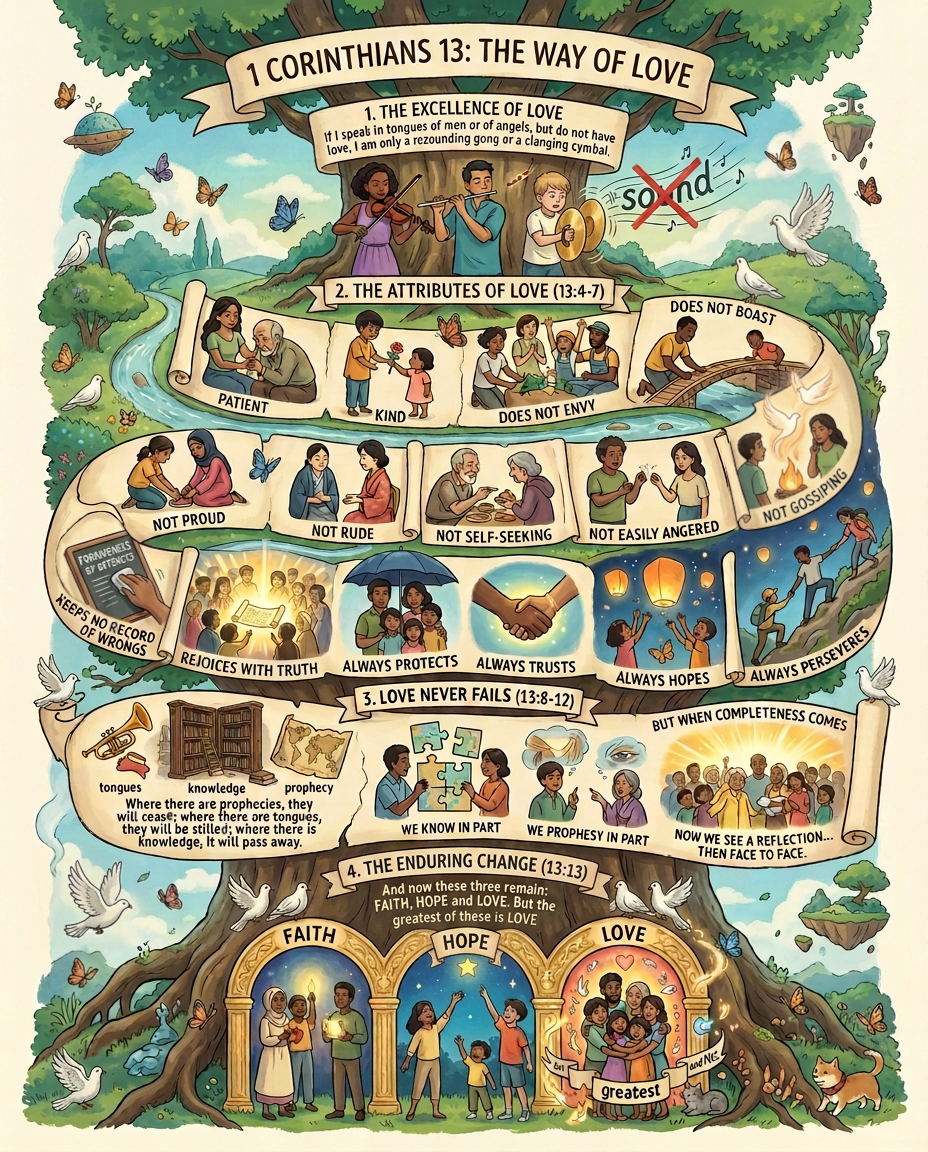
\includepdf[pages=1, fitpaper=false, width=\paperwidth, height=\paperheight, , keepaspectratio=false]{1corinthians_love.png}

%1 CORINTHIANS 14
\mychapter{} \myverse*{}Follow after love and earnestly desire spiritual gifts, but especially
that you may prophesy.
\myverse{}For he who speaks in another language speaks not to men, but to God, for no
one understands, but in the Spirit he speaks mysteries.
\myverse{}But he who prophesies speaks to men for their edification, exhortation, and
consolation.
\myverse{}He who speaks in another language edifies himself, but he who prophesies edifies
the assembly.
\myverse{}Now I desire to have you all speak with other languages, but even more that
you would prophesy. For he is greater who prophesies than he who speaks with other languages, unless he
interprets, that the assembly may be built up.

\myverse{}But now, brothers,\footnote{14:6 The word for “brothers” here and where context allows may also be correctly translated “brothers
	and sisters” or “siblings.”
} if I come to you speaking with other languages, what would I profit you unless I speak to you
either by way of revelation, or of knowledge, or of prophesying, or of teaching?
\myverse{}Even lifeless things that make a sound, whether pipe or harp, if they didn’t
give a distinction in the sounds, how would it be known what is piped or harped?
\myverse{}For if the shofar gave an uncertain sound, who would prepare himself for war?
\myverse{}So also you, unless you uttered by the tongue words easy to understand, how
would it be known what is spoken? For you would be speaking into the air.
\myverse{}There are, it may be, so many kinds of languages in the world, and none of
them is without meaning.
\myverse{}If then I don’t know the meaning of the language, I would be to him who speaks
a foreigner, and he who speaks would be a foreigner to me.
\myverse{}So also you, since you are zealous for spiritual gifts, seek that you may
abound to the building up of the assembly.

\myverse{}Therefore let him who speaks in another language pray that he
may interpret.
\myverse{}For if I pray in another language, my spirit prays, but my understanding
is unfruitful.

\myverse{}What should I do? I will pray with the spirit, and I will pray
with the understanding also. I will sing with the spirit, and I will sing with the understanding also.
\myverse{}Otherwise, if you bless with the spirit, how will he who fills the place
of the unlearned say the “Amen” at your giving of thanks, seeing he doesn’t know what you say?
\myverse{}For you most certainly give thanks well, but the other person is not built
up.
\myverse{}I thank my God, I speak with other languages more than you all.
\myverse{}However, in the assembly I would rather speak five words with my understanding,
that I might instruct others also, than ten thousand words in another language.

\myverse{}Brothers, don’t be children in thoughts, yet in malice be babies,
but in thoughts be mature.
\myverse{}In the law it is written, “By men of strange languages and by the lips of
strangers I will speak to this people. They won’t even listen to me that way, says the Lord.”\footnote{14:21 Isaiah 28:11-12}
\myverse{}Therefore other languages are for a sign, not to those who believe, but to
the unbelieving; but prophesying is for a sign, not to the unbelieving, but to those who believe.
\myverse{}If therefore the whole assembly is assembled together and all speak with
other languages, and unlearned or unbelieving people come in, won’t they say that you are crazy?
\myverse{}But if all prophesy, and someone unbelieving or unlearned comes in, he is
reproved by all, and he is judged by all.
\myverse{}And thus the secrets of his heart are revealed. So he will fall down on his
face and worship God, declaring that God is among you indeed.

\myverse{}What is it then, brothers? When you come together, each one
of you has a psalm, has a teaching, has a revelation, has another language, or has an interpretation.
Let all things be done to build each other up.
\myverse{}If any man speaks in another language, let there be two, or at the most three,
and in turn; and let one interpret.
\myverse{}But if there is no interpreter, let him keep silent in the assembly, and
let him speak to himself and to God.
\myverse{}Let two or three of the prophets speak, and let the others discern.
\myverse{}But if a revelation is made to another sitting by, let the first keep silent.
\myverse{}For you all can prophesy one by one, that all may learn and all may be exhorted.
\myverse{}The spirits of the prophets are subject to the prophets,
\myverse{}for God is not a God of confusion but of peace, as in all the assemblies
of the holy ones.
\myverse{}Let the wives be quiet in the assemblies, for it has not been permitted for
them to be talking except in submission, as the law also says,\footnote{14:34 Deuteronomy 27:9}
\myverse{}if they desire to learn anything. “Let them ask their own husbands at home,
for it is shameful for a wife to be talking in the assembly.”
\myverse{}What!? Was it from you that the word of God went out? Or did it come to you
alone?

\myverse{}If any man thinks himself to be a prophet or spiritual, let
him recognize the things which I write to you, that they are the commandment of the Lord.
\myverse{}But if anyone is ignorant, let him be ignorant.

\myverse{}Therefore, brothers, desire earnestly to prophesy, and don’t
forbid speaking with other languages.
\myverse{}Let all things be done decently and in order.


% 1 CORINTHIANS 15
\mychapter{} \myverse*{}Now I declare to you, brothers, the Good News which I preached
to you, which also you received, in which you also stand,
\myverse{}by which also you are saved, if you hold firmly the word which I preached to
you—unless you believed in vain.

\myverse{}For I delivered to you first of all that which I also received:
that Messiah died for our sins according to the Scriptures,
\myverse{}that he was buried, that he was raised on the third day according to the Scriptures,
\myverse{}and that he appeared to Kefa, then to the twelve.
\myverse{}Then he appeared to over five hundred brothers at once, most of whom remain
until now, but some have also fallen asleep.
\myverse{}Then he appeared to Jacob, then to all the emissaries,
\myverse{}and last of all, as to the child born at the wrong time, he appeared to me
also.
\myverse{}For I am the least of the emissaries, who is not worthy to be called an emissary,
because I persecuted the assembly of God.
\myverse{}But by the grace of God I am what I am. His grace which was given to me was
not futile, but I worked more than all of them; yet not I, but the grace of God which was with me.
\myverse{}Whether then it is I or they, so we proclaim, and so you believed.

\myverse{}Now if Messiah is preached, that he has been raised from the
dead, how do some among you say that there is no resurrection of the dead?
\myverse{}But if there is no resurrection of the dead, neither has Messiah been raised.
\myverse{}If Messiah has not been raised, then our proclaiming is in vain and your
faith also is in vain.
\myverse{}Yes, we are also found false witnesses of God, because we testified about
God that he raised up Messiah, whom he didn’t raise up if it is true that the dead are not raised.
\myverse{}For if the dead aren’t raised, neither has Messiah been raised.
\myverse{}If Messiah has not been raised, your faith is vain; you are still in your
sins.
\myverse{}Then they also who are fallen asleep in Messiah have perished.
\myverse{}If we have only hoped in Messiah in this life, we are of all men most pitiable.

\myverse{}But now Messiah has been raised from the dead. He became the
first fruit of those who are asleep.
\myverse{}For since death came by man, the resurrection of the dead also came by man.
\myverse{}For as in Adam all die, so also in Messiah all will be made alive.
\myverse{}But each in his own order: Messiah the first fruits, then those who are Messiah’s
at his coming.
\myverse{}Then the end comes, when he will deliver up the Kingdom to God the Father,
when he will have abolished all rule and all authority and power.
\myverse{}For he must reign until he has put all his enemies under his feet.
\myverse{}The last enemy that will be abolished is death.
\myverse{}For, “He put all things in subjection under his feet.”\footnote{15:27 Psalms 8:6} But when he says, “All things are put in subjection”,
it is evident that he is excepted who subjected all things to him.
\myverse{}When all things have been subjected to him, then the Son will also himself
be subjected to him who subjected all things to him, that God may be all in all.

\myverse{}Or else what will they do who are immersed for the dead? If
the dead aren’t raised at all, why then are they immersed for the dead?
\myverse{}Why do we also stand in jeopardy every hour?
\myverse{}I affirm, by the boasting in you which I have in Messiah Yeshua our Lord,
I die daily.
\myverse{}If I fought with animals at Ephesus for human purposes, what does it profit
me? If the dead are not raised, then “let’s eat and drink, for tomorrow we die.”\footnote{15:32 Isaiah 22:13}
\myverse{}Don’t be deceived! “Evil companionships corrupt good morals.”
\myverse{}Wake up righteously and don’t sin, for some have no knowledge of God. I say
this to your shame.

\myverse{}But someone will say, “How are the dead raised?” and, “With
what kind of body do they come?”
\myverse{}You foolish one, that which you yourself sow is not made alive unless it
dies.
\myverse{}That which you sow, you don’t sow the body that will be, but a bare grain,
maybe of wheat, or of some other kind.
\myverse{}But God gives it a body even as it pleased him, and to each seed a body of
its own.
\myverse{}All flesh is not the same flesh, but there is one flesh of men, another flesh
of animals, another of fish, and another of birds.
\myverse{}There are also celestial bodies and terrestrial bodies; but the glory of
the celestial differs from that of the terrestrial.
\myverse{}There is one glory of the sun, another glory of the moon, and another glory
of the stars; for one star differs from another star in glory.

\myverse{}So also is the resurrection of the dead. The body is sown perishable;
it is raised imperishable.
\myverse{}It is sown in dishonor; it is raised in glory. It is sown in weakness; it
is raised in power.
\myverse{}It is sown a natural body; it is raised a spiritual body. There is a natural
body and there is also a spiritual body.

\myverse{}So also it is written, “The first man Adam became a living soul.”\footnote{15:45 Genesis 2:7} The last Adam became a life-giving spirit.
\myverse{}However, that which is spiritual isn’t first, but that which is natural,
then that which is spiritual.
\myverse{}The first man is of the earth, made of dust. The second man is the Lord from
heaven.
\myverse{}As is the one made of dust, such are those who are also made of dust; and
as is the heavenly, such are they also that are heavenly.
\myverse{}As we have borne the image of those made of dust, let’s\footnote{15:49 NU, TR read “we will” instead of “let’s”} also bear the image of the heavenly.
\myverse{}Now I say this, brothers,\footnote{15:50 The word for “brothers” here and where context allows may also be correctly translated “brothers
	and sisters” or “siblings.”} that flesh and blood can’t inherit God’s Kingdom; neither does the
perishable inherit imperishable.

\myverse{}Behold,\footnote{15:51 “Behold”, from “ἰδοὺ”, means look at, take notice, observe, see, or gaze at. It is often used
	as an interjection.} I tell you a mystery. We will not all sleep, but we will all be changed,
\myverse{}in a moment, in the twinkling of an eye, at the last shofar. For the shofar
will sound and the dead will be raised incorruptible, and we will be changed.
\myverse{}For this perishable body must become imperishable, and this mortal must put
on immortality.
\myverse{}But when this perishable body will have become imperishable, and this mortal
will have put on immortality, then what is written will happen: “Death is swallowed up in victory.”\footnote{15:54 Isaiah 25:8}

\myverse{}“Death, where is your sting?

Sheol,\footnote{15:55 or, Hell} where is your victory?”\footnote{15:55 See
	Hosea 13:14}

\myverse{}The sting of death is sin, and the power of sin is the law.
\myverse{}But thanks be to God, who gives us the victory through our Lord Yeshua the Messiah.
\myverse{}Therefore, my beloved brothers, be steadfast, immovable, always abounding
in the Lord’s work, because you know that your labor is not in vain in the Lord.


% 1 CORINTHIANS 16
\mychapter{} \myverse*{}Now concerning the collection for the holy ones: as I commanded
the assemblies of Galatia, you do likewise.
\myverse{}On the first day of every week, let each one of you save as he may prosper,
that no collections are made when I come.
\myverse{}When I arrive, I will send whoever you approve with letters to carry your gracious
gift to Jerusalem.
\myverse{}If it is appropriate for me to go also, they will go with me.

\myverse{}I will come to you when I have passed through Macedonia, for I
am passing through Macedonia.
\myverse{}But with you it may be that I will stay with you, or even winter with you,
that you may send me on my journey wherever I go.
\myverse{}For I do not wish to see you now in passing, but I hope to stay a while with
you, if the Lord permits.
\myverse{}But I will stay at Ephesus until Shavu`ot,
\myverse{}for a great and effective door has opened to me, and there are many adversaries.

\myverse{}Now if Timothy comes, see that he is with you without fear,
for he does the work of the Lord, as I also do.
\myverse{}Therefore let no one despise him. But set him forward on his journey in peace,
that he may come to me; for I expect him with the brothers.

\myverse{}Now concerning Apollos the brother, I strongly urged him to
come to you with the brothers, but it was not at all his desire to come now; but he will come when he
has an opportunity.

\myverse{}Watch! Stand firm in the faith! Be courageous! Be strong!
\myverse{}Let all that you do be done in love.

\myverse{}Now I beg you, brothers—you know the house of Stephanas, that
it is the first fruits of Achaia, and that they have set themselves to serve the holy ones—
\myverse{}that you also be in subjection to such, and to everyone who helps in the
work and labors.
\myverse{}I rejoice at the coming of Stephanas, Fortunatus, and Achaicus; for that
which was lacking on your part, they supplied.
\myverse{}For they refreshed my spirit and yours. Therefore acknowledge those who are
like that.

\myverse{}The assemblies of Asia greet you. Aquila and Priscilla greet
you warmly in the Lord, together with the assembly that is in their house.
\myverse{}All the brothers greet you. Greet one another with a holy kiss.

\myverse{}This greeting is by me, Paul, with my own hand.
\myverse{}If any man doesn’t love the Lord Yeshua the Messiah, let him be cursed.\footnote{16:22 Greek: anathema.} Come, Lord!\footnote{16:22 Aramaic: Maranatha!}
\myverse{}The grace of the Lord Yeshua the Messiah be with you.
\myverse{}My love to all of you in Messiah Yeshua. Amen.


